\section{Обработка табличных данных. Часть 2 }

\subsection{Условие задания}
Разработать приложение в соответствии со своим вариантом. Номер задания выбирается преподавателем.

Проверить работу приложения на приведенных тестовых примерах.

\textbf{ЗАДАНИЕ ПРЕДПОЛАГАЕТ НАЛИЧИЕ ДВУХ ТАБЛИЦ.} В  первую вводятся данные (должна быть проверка, что введены цифры). Вторую лучше сделать доступной только для чтения. В нее записывается результат. 

\textbf{ФРАЗА "ЗАМЕНИТЬ СТРОКОЙ X"  предполагает, что создается либо таблица, состоящая из одной строки и туда вводятся данные, либо создается текстовое поле, куда вводится число, и вся строка таблицы заменяется этим числом.}

\textbf{ДИАПАЗОН [a,b] означает, что mas[i][j] >= a \&\& mas[i][j] <= b.}

Приложение должно содержать следующие компоненты:
\begin{enumerate}
    \item Заголовок формы должен отражать суть задания.
    \item Все элементы формы должны быть внятно подписаны (кнопки подписаны, у текстового поля должно быть написано, для чего оно нужно и т. д.)
    \item В коде должны быть комментарии и отступы (код должен быть легко читаем).
    \item  Таблица может быть задана двумя способами: 
    \begin{itemize}
        \item либо ввести количество строк и столбцов (тогда необходима проверка, что введено не число) и создать нужную таблицу. При изменении количества строк и столбцов, старая таблица должна быть удалена.
        \item либо добавлять и удалять строки и столбцы с помощью отдельных кнопок. Проследить, чтобы приложение не завершалось аварийно (не удалять нулевую строку).
    \end{itemize}
    \item  Должна быть проверка ошибок - ввод не числа, ввод числа, приводящего к переполнению стека или выхода результата за границы диапазона типа. В таблице также должны быть введены целые числа. В случае ошибочного ввода поля результатов должны автоматически очищаться.
    \item Если данные введены корректно, но отсутствуют необходимые данные (например, надо найти сумму нечетных чисел, а в таблице только четные), то в поле результата должно быть выведено об этом сообщение.
    \item В случае задач с вводом диапазона [a,b] необходима обязательная проверка, что a < b.
\end{enumerate}

\textbf{Вариант 12.} Смотреть на рисунке \ref{task5_var12}.
\begin{figure}[H]
    \centering
    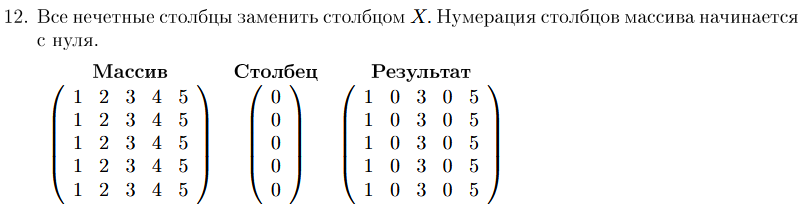
\includegraphics[width=0.9\linewidth]{lections/img/task5_var12.png}
    \caption{Задание 5 Вариант 12}
    \label{task5_var12}
\end{figure}

\subsection{Вид формы в конструкторе}


Создано окно приложения, содержащее два элемента TextBox, три элемента Label, шесть элементов Button, три элемента gridview (один из которых содержит атрибут ReadOnly) и один элемент ErrorProvider для обработки ошибок. Вид окна представлен на рисунке \ref{task5_form} \cite{лафоре2011объектно}.
\begin{figure}[H]
    \centering
    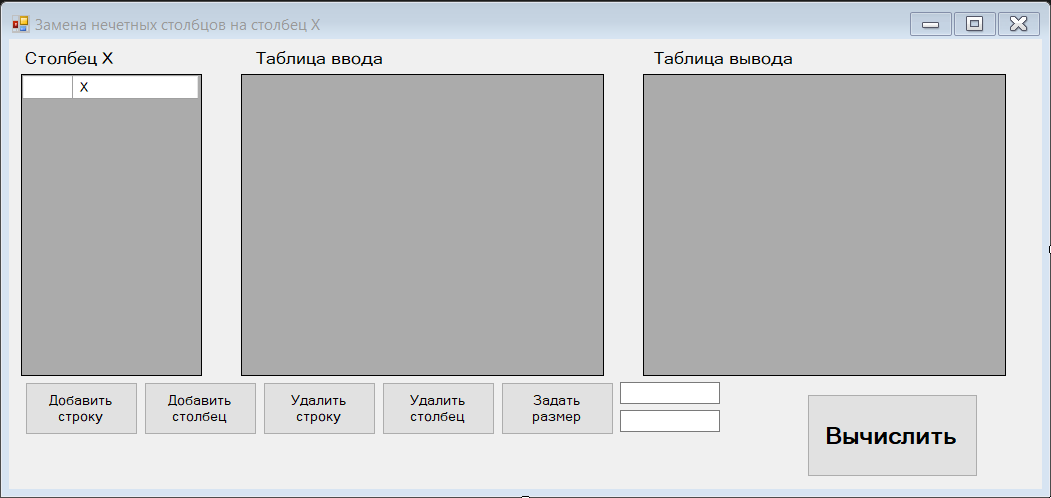
\includegraphics[width=1\linewidth]{lections/img/task5_form.png}
    \caption{Окно приложения «Обработка табличных данных. Часть 2» открытое в конструкторе}
    \label{task5_form}
\end{figure}


\subsection{Таблица с описанием переименованных элементов формы}
Все измененные элементы формы указаны в таблице \ref{task5_attributes}.

\begin{table}[H]
\caption{Значения атрибутов элементов в приложении <<Обработка табличных данных. Часть 2>>}
\begin{tabular}{|l|l|l|}
\hline
\textbf{\begin{tabular}[c]{@{}l@{}}Описание элементов\\ формы\end{tabular}}      & \textbf{\begin{tabular}[c]{@{}l@{}}Список измененных\\ атрибутов\end{tabular}} & \textbf{\begin{tabular}[c]{@{}l@{}}Новое значение\\ атрибута\end{tabular}}    \\ \hline
Форма MyForm                                                                     & Text                                                                           & \begin{tabular}[c]{@{}l@{}}Обработка табличных\\ данных. Часть 2\end{tabular} \\ \hline
\begin{tabular}[c]{@{}l@{}}TextBox ввода количества\\ строк таблицы\end{tabular} & Name                                                                           & set\_size\_lines                                                              \\ \hline
\begin{tabular}[c]{@{}l@{}}TextBox ввода количества\\ Столбцов таблицы\end{tabular} & Name                                                                           & set\_size\_columns                                                            \\ \hline
TextBox ввода конца интервала                                                    & Name                                                                           & int\_b                                                                        \\ \hline
\multirow{2}{*}{TextBox вывода кратных х}                                        & Name                                                                           & krat\_box                                                                     \\ \cline{2-3} 
                                                                                 & ReadOnly                                                                       & True                                                                          \\ \hline
\multirow{2}{*}{TextBox вывода минимума}                                         & Name                                                                           & chet\_box                                                                     \\ \cline{2-3} 
                                                                                 & ReadOnly                                                                       & True                                                                          \\ \hline
\multirow{2}{*}{Кнопка "Добавить строку"}                                        & Name                                                                           & Add\_line                                                                     \\ \cline{2-3} 
                                                                                 & Text                                                                           & Добавить строку                                                               \\ \hline
\multirow{2}{*}{Кнопка "Добавить столбец"}                                       & Name                                                                           & add\_column                                                                   \\ \cline{2-3} 
                                                                                 & Text                                                                           & Добавить столбец                                                              \\ \hline
\multirow{2}{*}{Кнопка "Удалить строку"}                                         & Name                                                                           & remove\_line                                                                  \\ \cline{2-3} 
                                                                                 & Text                                                                           & Удалить строку                                                                \\ \hline
\multirow{2}{*}{Кнопка "Удалить столбец"}                                        & Name                                                                           & remove\_column                                                                \\ \cline{2-3} 
                                                                                 & Text                                                                           & Удалить столбец                                                               \\ \hline
\multirow{2}{*}{Кнопка "Задать размер"}                                          & Name                                                                           & set\_size                                                                     \\ \cline{2-3} 
                                                                                 & Text                                                                           & Задать размер                                                                 \\ \hline
\multirow{2}{*}{Кнопка "Вычислить"}                                              & Name                                                                           & solve\_btn                                                                    \\ \cline{2-3} 
                                                                                 & Text                                                                           & Вычислить                                                                     \\ \hline
\multirow{3}{*}{Таблица ввода столбца X}                                         & Name                                                                           & X\_input                                                                      \\ \cline{2-3} 
                                                                                 & AllowUserToAddRows                                                             & False                                                                         \\ \cline{2-3} 
                                                                                 & AllowUserToDeleteRows                                                          & False                                                                         \\ \hline
\multirow{3}{*}{Таблица ввода матрицы}                                           & Name                                                                           & input\_grid                                                                   \\ \cline{2-3} 
                                                                                 & AllowUserToAddRows                                                             & False                                                                         \\ \cline{2-3} 
                                                                                 & AllowUserToDeleteRows                                                          & False                                                                         \\ \hline
\multirow{4}{*}{Таблица вывода}                                                  & Name                                                                           & output\_grid                                                                  \\ \cline{2-3} 
                                                                                 & AllowUserToAddRows                                                             & False                                                                         \\ \cline{2-3} 
                                                                                 & AllowUserToDeleteRows                                                          & False                                                                         \\ \cline{2-3} 
                                                                                 & ReadOnly                                                                       & True                                                                          \\ \hline
\end{tabular}
\label{task5_attributes}
\end{table}


\subsection{Примеры правильной и неправильной работы}
После запуска программы на экране появляется окно на рисунке \ref{task5_launch1}.
\begin{figure}[H]
    \centering
    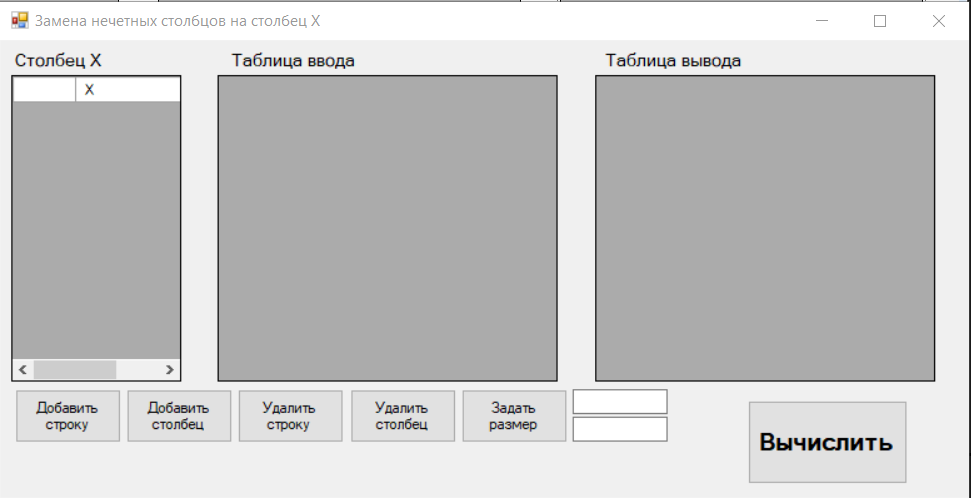
\includegraphics[width=1\linewidth]{lections/img/task5_launch1.png}
    \caption{Запуск программы}
    \label{task5_launch1}
\end{figure}

После ввода столбца X и таблицы ввода и нажатии на кнопку "Вычислить" (на рисунке \ref{task5_launch2}).

\begin{figure}[H]
    \centering
    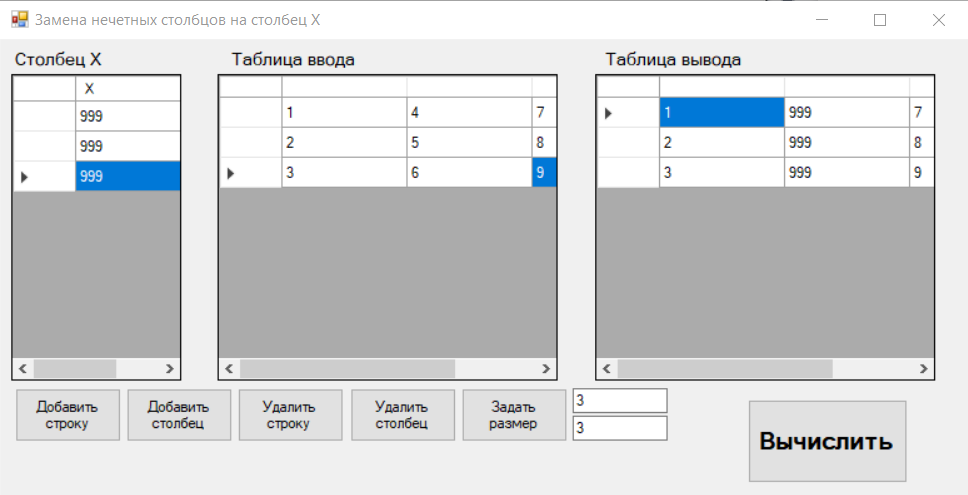
\includegraphics[width=1\linewidth]{lections/img/task5_launch2.png}
    \caption{Замена всех нечетных столбцов столбцом Х (счет начиется с 0)}
    \label{task5_launch2}
\end{figure}

При попытке ввода не числа в таблицу, программа выведет ошибку (на рисунке \ref{task5_launch3})
\begin{figure}[H]
    \centering
    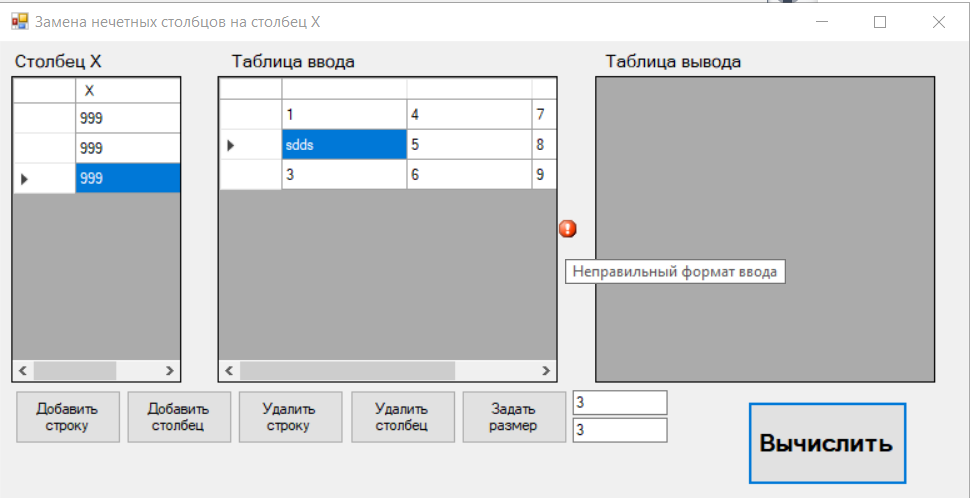
\includegraphics[width=1\linewidth]{lections/img/task5_launch3.png}
    \caption{Ошибка формата ввода}
    \label{task5_launch3}
\end{figure}



\subsection{Примеры исходного кода}


Функция при нажатии на кнопку "Удалить столбец".
\begin{minted}[style=bw,
 linenos=true,
 breaklines=true,
 numbersep=5pt,
 tabsize=2,
 fontsize=\small,
 bgcolor=white]{cpp}
private: System::Void remove_column_Click(System::Object^ sender, System::EventArgs^ e) {
	this->errorProvider1->Clear();
	if (this->input_grid->ColumnCount <= 1 || this->input_grid->RowCount == 0) {
		this->errorProvider1->SetError(remove_column, "Нельзя убрать столбец, которого нет");
		return;
	}
	int i = this->input_grid->CurrentCell->ColumnIndex;
	this->input_grid->Columns->Remove(this->input_grid->Columns[i]);
}
\end{minted}
Другие фрагменты кода расположены в приложении \ref{app:table_data_2}.

\sectionbreak